\documentclass[letterpaper,12pt,fullpage]{article}

\usepackage[left=1in,right=1in,top=1in,bottom=1in]{geometry}
\usepackage{cite}
\usepackage{graphicx}
% \usepackage[dvips]{graphicx}
% \usepackage{epsfig} % for postscript graphics files
  % \graphicspath{{../eps/}}
% \DeclareGraphicsExtensions{.eps}
\usepackage{amsmath}
\usepackage{amssymb}
%\usepackage[cmex10]{amsmath}
%\usepackage{array}
%\usepackage{mdwmath}
%\usepackage{mdwtab}
%\usepackage{eqparbox}
\usepackage[tight,footnotesize]{subfigure}
%\usepackage[caption=false]{caption}
%\usepackage[font=footnotesize]{subfig}
%\usepackage{fixltx2e}
%\usepackage{stfloats}
\usepackage{hyperref}

% correct bad hyphenation here
%\hyphenation{op-tical net-works semi-conduc-tor}

\input latex-commands

\begin{document}

\title{A Survey of Near-Term Exoskeleton Technology\\
(Draft 3.0)}

\author{Alex Ansari, Christopher G. Atkeson, Howie Choset, and Matthew Travers\\
Carnegie Mellon University}

\maketitle

\begin{abstract}
Abstract to be written.
\end{abstract}

\section{Executive Summary}

Executive Summary to be written.

\section{Scope: What is this paper about?}

This paper surveys near-term exoskeleton technology with an
emphasis on control.
A companion paper surveys implemented exoskeleton technology [survey.pdf].

The focus is on near-term exoskeleton technologies that allow a
highly trained and top percentile athletic 
operator to carry a payload that weighs approximately the same amount
as the operator. We envisage these types of exoskeletons to be useful
in carrying protective and safety equipment for SWAT teams, police,
firefighters, and soldiers. 

We do not survey exoskeleton technology for human arms. 
We treat the torso and helmet of the exoskeleton as the payload,
and focus on a lower body exoskeleton to support any payloads that
are on the torso or head.

We do not cover global energy storage such as batteries or liquid fuel
or other global power system issues.

A later white paper could discuss the use of propulsive forces other
than foot contacts, as well as additional actuation at the contacts (air
bags, springs, other ways to rapidly apply stored energy) for
operator safety (dodging threats, ...) and high performance (jumping, ...).

A future white paper could discuss near term soft robotics technology
for exoskeletons.

A future white paper could discuss the addition of extra limbs and
other effectors to an exoskeleton~\cite{IEEE07139896}.

%%%%%%%%%%%%%%%%%%%%%%%%%%%%

%\section{What are some design philosophy alternatives?}

\subsection{``Invisible'' exoskeleton}

Can we build an exoskeleton allows the operator to behave naturally
and exerts little or no force on the operator?

This design goal
could be achieved through active control using feedback of the
operator-exoskeleton forces and/or high quality prediction of what
the operator will do next. Additional gravity, friction, actuator, and
inertial compensation (inverse dynamics) can improve performance.

\subsection{``Natural'' exoskeleton}

Can we build an exoskeleton allows the operator to behave naturally?
The operator can feel the exoskeleton, but can overpower it when necessary.

One way to achieve this design goal is to have extremely light attachments
to the limbs, and put all heavy exoskeleton components on the
torso and head. The limbs can be physically driven by the operators muscles
with little ``drag'' on the operator.
Bypass valves and clutches could allow the operator to physically ``take over''
and push the relatively lightweight limb mounted parts of the exoskeleton around.

A complementary way to achieve this goal is through active control. Low impedance
(torque source) actuation makes combining active control with operator backdriving
easier.

A ``natural'' exoskeleton is easier to build than 
an ``invisible'' exoskeleton.

\subsection{``Symbiotic'' exoskeleton}

Can we build an exoskeleton that allows the operator/exoskeleton team
to be effective, but not necessarily behave naturally? 
The operator needs to learn to ``fly'' the suit,
just as operators learn to operate parachutes,
wing suits, diving equipment, high and low temperature protective
suits, firefighting equipment, and high altitude flight
and parachute suits.

An advantage of this approach is that 
the exoskeleton can adapt its behavior to the task.
For example, for jumping, the exoskeleton can operate like a pogo 
stick:\\
\url{https://www.youtube.com/watch?v=lbp41vWP4o4},\\ 
and for running it could act like jumping stilts:\\
\url{https://www.youtube.com/watch?v=9ZOd7yEyhwI},

A ``symbiotic'' exoskeleton is easier to build than an ``invisible'' or ``natural''
exoskeleton.


%%%%%%%%%%%%%%%%%%%%%%%%%%%%

\section{Specifications}

We would like to find actuation that can keep up with human
speeds and provide forces or torques comparable to human capabilities:
\begin{enumerate}
\item
2-4 revolutions/second maximum joint speed.
\item
200-400Nm maximum torque at a joint.
\end{enumerate}

{\it Dennis E. Anderson, Michael L. Madigan, Maury A. Nussbaum,
“Maximum voluntary joint torque as a function of joint angle and
angular velocity: Model development and application to the lower
limb”, Journal of Biomechanics, 2007, Volume. 40, Issue 14, Pages
3105-3113} says max knee torque is around 350Nm. They only consider
max knee angular velocities around 2revolutions/second.

\section{What performance is currently available?}

\subsection{Reference Design: linear hydraulic with bypass valves}

This section considers hydraulics using linear actuators (pistons).
It is possible that rotary hydraulics, such as vane motors,
can do better, but we are not aware of non-proprietary examples
to discuss.

\subsubsection{What limits performance?}

The differential pressure of the hydraulic fluid supply vs.\ the fluid
return limits the maximum force. Pressure times piston cross-sectional area
determines actuator force.
Many components are rated for 3000psi = 207bar (usually approximated to
210bar).
(Units: 1 bar = $10^5$ newtons per square meter (pascals) = 14.5 psi).

The flow capacity of the hydraulic fluid supply and return limits
the maximum speed. Linear velocity*piston cross-sectional area determines 
the fluid flow required.
(Units: 1 lpm = 0.264 gpm)

The power capacity of the hydraulic pump determines the maximum force
at a given flow rate.

To power our SARCOS Primus Humanoid Robot we use an
MTS SilentFlo Hydraulic Power Unit (HPU) 515.11
which operates at 3000psi $\approx$ 210bar,
has a maximum flow of 41.6lpm = 11gpm, and is rated at
18.5 kW = 25hp.

There is also a thermal limit. Hydraulic systems heat up during operation,
and there must be cooling (air or water cooling is often used)
applied somewhere in the system. Heat is transferred by the flowing oil,
so both the HPU, the piping and hoses, and the valves and actuators get hot.

The flow capacity of a hydraulic valve also limits the maximum flow.
The MOOG Type 30 Series 30 Nozzle-Flapper Flow Control Servovalves
are popular on hydraulic humanoids. Their maximum flow is
12lpm = 3.1gpm at 3000psi $\approx$ 210bar.
You might want to get a higher capacity valve. To do this, you
would sacrifice valve bandwidth and flow leakage.
The bandwidth of the MOOG Type 30
Series 30 is about 200Hz, and the leakage ranges from
0.3 to 3gpm. Leakage in this case is internal to the hydraulic
system, from the valve fluid supply port to the valve fluid return port.
Valve leakage is flow and thus power and force
not available to the actuation.
A humanoid robot might have 30 of these valves,
so it would not take a lot of leakage per valve to completely
use up the flow capacity of the HPU.

The size and weight of an HPU, and how to power it are limiting.
There have been examples of portable HPUs driven by electric and IC motors.
The Atlas humanoid
robot had an HPU driven by batteries (don't have specs).
Max pressure was around 2600psi.
We have specifications for a portable 
5kW HPU with 4gpm at 3000psi; 170V, 30A input; weighing
40lb and 15x10x10in in size.
A heat exchanger is an additional 14x28x6in in size.
Batteries to power this would be also take up space and 
add weight.

\subsubsection{A reference design}

A linear hydraulic actuator (a piston, for example) has a cross sectional
area ($A$) and a moment arm ($M$). Maximum torque of a single actuator
is $P*A*M$ where $P$ is the operating pressure.
Maximum velocity is $F/(A*M)$ where $F$ is the maximum flow at the
actuator.
Flow, unfortunately, is divided across multiple actuators,
so more moving actuators would reduce this limit.

Here is a simple actuator design:
\begin{equation}
A = 10cm^2 = 10^{-3}m^2, \; \; \; M = 0.01m
\end{equation}
Maximum torque is
\begin{equation}
P*A*M = 210*10^5N*m^{-2}*10^{-3}m^2*0.01m = 210Nm 
\end{equation}
Maximum angular velocity is
\begin{equation}
F/(A*M) = 0.2lps*(1000cm^3/l)/(10cm^2*1cm) = 20r/s = 3.2rev/s
\end{equation}

The Sarcos Primus Humanoid (which uses the MOOG valve described
above) and the Atlas humanoid (which uses similar custom MOOG valves)
are both designed
for maximum joint velocities of about 2 revolutions/second (12.5radians/s).
and generate joint torques of up to around 400Nm.
Doubling the maximum speed would half the maximum torque, which matches
our simple actuator design.

\subsubsection{What have we learned from implementations?}

High performance force control has been demonstrated many times
on many hydraulic robots (Sarcos, Atlas, HyQ, ...)

However, on the Atlas robot differential oil pressure is used
to estimate actuator force, as this form of force sensing
is quite mechanically robust (low maintenance).
This measurement is before the piston
seals and transmission, so it does not capture those sources
of friction. The joint torques are off by up to 10Nm at each joint.
The Sarcos robot uses load cells in the actuator to joint transmissions.

On the Atlas humanoid robot there was electromagnetic interactions between
nearby valves.

\subsubsection{Can we do better?}

Can we expect major improvements in hydraulics?
There has been incremental improvement on HPUs and valves since
the 1950s. Rapid prototyping and 3D printing are leading to
easier integration of valves, actuators, and sensors (see following
paragraph). Current high performance valves are flow control valves. It
is possible that lower leakage valves could be developed. It is possible
that pressure control valves would reduce the need for high bandwidth
force control, and thus high bandwidth valves. Pressure control valves
could also greatly improve exoskeleton safety if pressure control was
implemented physically rather than computationally, since physical
mechanisms are less likely to ``go unstable''.
Bypass mechanisms (a form of clutch) would allow hydraulic systems
to be backdriven without oil flow at high force, which would reduce
the power load on the HPU and the need for high performance force control.
Any valves or additional hydraulic circuitry
would have to have low internal leakage, and previous attempts at
pressure control valves have had leakage problems.
Gear shifts and variable transmissions would allow the maximum torque
and maximum no-load speed of the joint to be increased (also true
for all other actuation types).

{\bf Integrated Moog hydraulic actuator:}
Moog is developing an integrated hydraulic actuator with built-in
sensors and valves. Our colleagues report:
{\it The integrated Moog system is still very experimental,� there are
only two working prototypes right now.� Our lab is working closely
with Moog to develop the firmware for the builtin controllers. I
think it is a little early to say how well they work, but it looks
promising.}
\url{http://www.designnews.com/document.asp?doc_id=277754&dfpPParams=ht_13,kw_robotics,kw_41,aid_277754&dfpLayout=article}

\subsection{Reference Design: rotary electric}

This section considers heavily geared rotary electric motors.

\subsubsection{What limits performance?}

Electric motors are much more flexible than hydraulics in terms of voltages
and currents, as there is not a standard voltage equivalent to the 3000psi
design point in hydraulics.

Ultimately, electric motors, gears, and other drive train elements such
as clutches and variable transmissions are limited by size and weight.

One limitation on electrical current
is thermal. Motors overheat and windings melt.
A typically 
higher limit on electrical current is demagnetization of motor magnets.

\subsubsection{A reference design}

The JST lab at the University of Tokyo pushed the design of water
cooled electric motors and motor drivers. This led to the high
performance of the Schaft robot, a spinoff from that lab.

The water cooled motor driver they developed is capable of 80V and
80A continuous.~\cite{IEEE05649683}

They modified
MAXON EC-powermax30 200W brush-less motors, and added harmonic drives
to make an integrated actuator.
The maximum speed of these actuators was 3 revolutions/second.
The maximum torque using 2 drivers/motor was theoretically 400Nm, but
we have only seen 300Nm in the published data. 2 rev/s can be achieved
at peak torque (Fig~\ref{f:s1}).~\cite{IEEE05649683}

\begin{figure}[t]
\centering
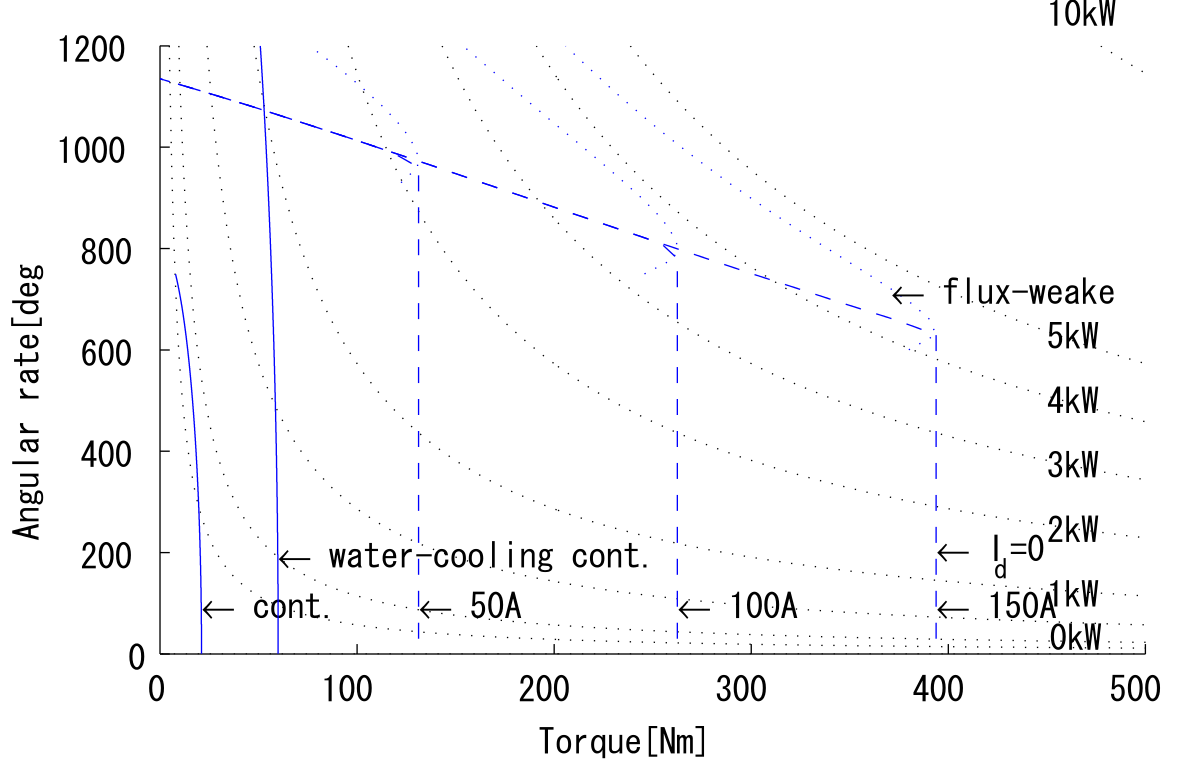
\includegraphics[width=0.75\textwidth]{tech-figs/s1}
\caption{Water cooled actuator capabilities.}
\label{f:s1}
\end{figure}

Peak currents are in the range of 100-150A.
{\it
``High current load on Li-ion or Ni-MH batteries affects life
span or cause damage. They cannot be charged with high
current rate. Electrical double layer capacitors are suitable for
such instantaneous current supply because they can supply
high current without degradation for high current while
their power capacity is not large. Capacitors can be charged
with high current. Combination of an electrical double layer
capacitor and battery is adopted. The robot carries a capacitor
developed for it by Shizuki Electric Co. Inc. Specifications of
the developed capacitor are shown in Tab.II.''}~\cite{IEEE05649683}
Note that this capacitor weighs 9 kg (Fig~\ref{f:s2}).

\begin{figure}[h]
\centering
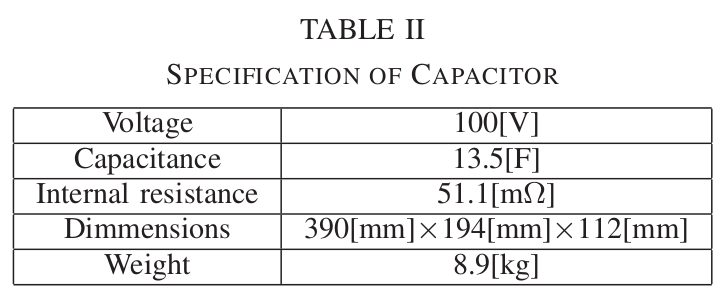
\includegraphics[width=0.75\textwidth]{tech-figs/s2}
\caption{Capacitor specifications.}
\label{f:s2}
\end{figure}

\subsubsection{What have we learned from implementations?}

This effort ``went dark'' after Google bought the spinoff company
Schaft, so there is a lot we don't know.

There are concerns about motor lifetime with this pattern of utilization.

This approach relies on transient loading of the motor, which needs
to be planned in advance to avoid not having thermal capacity
when more high performance is needed.
It is not clear how much this approach helps with 
steady state behaviors such as running.

Driving the motors this hard generates a lot of electromagnetic interference,
so they went with optical fiber for information transmission in their
robots.

We don't know whether these actuators can be made backdrivable with
high performance torque control. Pre-Schaft, the researchers were exploring
nonlinear series elastic actuation (big springs)
to help handle impacts and large force
transients~\cite{IEEE06651562}.

\subsubsection{Can we do better?}

This idea is a relatively new one, so there is probably useful unexplored
territory in the design space.

\section{Energy Storage}

We will only address energy storage
in terms of control issues. We are particularly interested in the
possibilities of joint-level or local energy storage.

Systems whose global energy storage is batteries waste
less energy driving electrical systems, but there are plenty of electrically
driven hydraulic systems on robots.
Systems whose global energy storage is liquid fuel (gasoline etc)
waste less energy driving a hydraulic system.

\subsection{Joint and synergy-level energy storage}

Can we use local energy storage to assist control: charging batteries or
supercapacitors, pressurizing accumulators, using springs, ... ?
The reference electrical design used a big capacitor to help handle
peak loads. We believe that many behaviors ``slosh'' potential and
kinetic energy back and forth.
Running exchanges vertical velocity and energy storage in spring-like
tissue.
Walking exchanges forward velocity and gravitational storage.
We also believe that energy storage can be used to start and stop
highly dynamic transient behaviors.
Jumping stilts and pogo sticks are an excellent demonstration
of the use of energy storage to enhance human
capabilities.
\url{https://www.youtube.com/watch?v=lbp41vWP4o4},
\url{https://www.youtube.com/watch?v=9ZOd7yEyhwI}

In addition, physical springs protect the exoskeleton from damage
and contribute to system dependability.
The JST lab was exploring human-scale jumping robots
with 
nonlinear series elastic actuation (big springs)
to help handle impacts and large force
transients~\cite{IEEE06651562}.

\section{Actuation}

What role do physical properties of actuation play in control? Highly
geared electric systems and hydraulic systems are inherently very
stiff and go where you want, but must be made compliant/backdrivable
using high performance (expensive and fragile) force control.
Pneumatics and Series Elastic Actuation (SEA) are inherently
compliant/backdrivable, which may reduce the performance
needed from the sensors and control system, but may not be able to
produce needed forces and speeds.

Here are some actuation types that have not been adequately explored
in humanoid robots and exoskeletons.

\subsection{Flywheels}

Energy storage and actuation for superhuman manueverability.
\url{http://www.ric.org/app/files/public/4898/LemusVallery_GyroscopicBackpack_EMBC2014pdf.pdf}
\url{http://www.ncbi.nlm.nih.gov/pubmed/22169384}


\subsection{Internal combustion actuators}

Several labs have explored using the piston of an internal combustion
engine as a stand-alone linear or rotary actuator. In this case
the combustion event would be carefully metered and timed. Repetitive
combustion events combined with mechanical filtering could lead to smooth
output forces. This approach inherits the desirable energy storage capacity
of liquid fuels. 
\url{http://softroboticstoolkit.com/book/combustion-driven-actuators}
\url{http://www.nature.com/articles/srep04296}
\url{http://arxiv.org/abs/1402.7101}
\url{http://ntrs.nasa.gov/archive/nasa/casi.ntrs.nasa.gov/20100021938.pdf}
% https://smartech.gatech.edu/bitstream/handle/1853/19873/warta_brett_j_200712_mast.pdf
\url{http://www.msoe.edu/servlet/JiveServlet/previewBody/5589-102-1-7785/Sarah_Swanson_Final_Paper.pdf}

\subsection{Hybrid actuation}

Different types of actuation can be combined: springs and electric motors,
for example. This combination can also be viewed as combining energy
storage and actuation. Slow pneumatics and fast electric motors~\cite{Morimoto,UCLA}.
Mini/Macro~\cite{Stanford}. In this view, the human operator is just
one more set of actuators to be added to the combined system.

We can consider the following combinaitons:
\begin{itemize}
\item
parallel combinations - fast but weak  actuator needs to hit joint limit and then be strong. (leads to chattering) or just lock in position to exert big force
\item
series combination - strong but slow actuator needs to clutch out of circuit to move fast
\end{itemize}

\section{How can clutches and gear shifts help?}

How can we implement a gear shifting system (the crucial mechanical
system missing in current robots)? How do we switch from manipulation
while standing, walking, running, other rapid movement (dodging), and
power movements (getting up from a squat or chair,
jumping, moving through doors and walls, pushing large objects
with full body while standing or seated)?

Examples:~\cite{IEEE07222598}

\section{Discussion}

{\bf Non-rigid systems:}
Light exoskeletons will have a lot of structural flexibility,
and will be poorly defined kinematically. This is not a
problem for applying forces, but it is a problem for determining
positions and velocities, such as center of mass position and velocity.

{\bf How exoskeleton attached to human:}
The human and exoskeleton limbs are typically connected to each
other with straps or padding. These connections typically have substantial
compliance and play, and may or may not have appropriate damping.
Typically the human and the exoskeleton do not move the same way:
pose, and linear and angular velocities and accelerations are not the same.

{\bf Heat exhaust:}
Will actuators, housing, and structure get too hot and fry operator?
Heatsink cooling, Force air cooling, Water cooling.
Hot material ejection.

{\bf Weight distribution:}
There is a weight distribution issue. Ideally the exoskeleton should
have a center of mass at the same location as the operator. Otherwise,
operator movements can be degraded and substantial forces occur between
the operator and the exoskeleton.
This constraint can be reduced with the use of propulsive forces other
than foot contacts: rockets (solid or liquid fuel), jets, exploding armor,
ducted fan air flow, ...

{\bf One Time Use:}
What happens if the suit is "one time use"? For example, ablative armor,
armor that reacts to incoming projectiles before they hit,
or explosive shielding could be used. Could the armor weight be decreased?
The expensive parts of the suit could be re-usable, and even autonomously
return to safe areas.

{\bf Do we need physical contact?}
Current exoskeletons use physical contact with the operator to control
the exoskeleton. Can we make an exoskeleton that does not touch or
minimally touches the operator, and in which there is no power
transfer between the operator and the exoskeleton? These types of
systems might allow an operator to behave more normally, have a
greater range of movement, be less tiring, and for non-enclosing
systems, allow the operator to move independently of the system (such
as aim and fire standard weapons or dive for cover) for additional
operator performance and safety.
\begin{enumerate}
\item
A "fat suit" or "sumo suit" could fully enclose the operator, but
use distance sensing to move with the operator.
\item
A "shield" could enclose the front of an operator (or whatever
portion of the operator is threatened) and move with the operator,
\item
A "human shield" (actually a machine shield) could move ahead of
an operator, mimicking the operators movement.
\item
An "angel" could walk, jump, or fly between an operator and potential
hostile sites, and deflect or disable projectiles.
\end{enumerate}

\section{Conclusions and Recommendations}

1) We recommend the exploration of how to implement and utilize practical
{\bf gear shifts and clutches} (or equivalents). For hydraulics and air, this might mean
bypass or other special valve features.
For electric motors and gears, this might mean special purpose clutch mechanisms
built into gearing or harmonic drives. For linear actuators, antagonistic actuation
combined with tendons that can go slack can be used for clutching.

2) We recommend exploring the combination of {\bf passive energy storage} (springs,
accumulators, supercapacitors, ...) with active actuation. One form of this
is series elastic actuation. 

3) We also recommend exploring storing energy with
a ``catch'' and ``explosive release'' for {\bf overdrive capabilities}. 

4) We recommend the exploration of {\bf hybrid actuation,} where strong but slow actuators
are combined with fast but weak actuators either in parallel or serial.

5) We recommend the exploration of {\bf multi-joint or synergy actuation}, where an actuator
might cross two or more joints.

6) We recommend the exploration of {\bf modular integrated sensing/actuation units} using 3D printing
or other rapid prototyping techniques, such as the integrated Moog hydraulic
actuator for HyQ.

7) We recommend applying {\bf as many sensors as possible,} and asking the performers
to make it easy to add more by making the sensor network available in the design.
This maximizes the probability of success
by enabling multiple control
approaches to be implemented, refined, and support each other.
In particular, we would like to see force sensing between the operator and the
exoskeleton, including at the feet, as much force sensing between the exoskeleton 
and the world as possible, but minimally full six-axis force/torque sensing at
the exoskeleton feet (where they touch the ground). We would like to see multiple MEMs
IMUs (measuring linear acceleration and angular velocity) installed across 
the exoskeleton and at least one high quality fiber optic gyro IMU.
We would like to see high quality direct velocity sensing
such as high count (100,000 counts/revolution) encoders and/or 
analog rotary or linear tachometers on actuators and joints. 
We would like to see actuator force or torque sensors
(load cells or equivalents) with the measurement on the link side (rather than
the actuator side) of any transmission. Electric current in motors and oil
pressure in hydraulic pistons can also be used for actuator force estimation,
but because these measurements are on the actuator side before the transmission
and in the case of hydraulics before the oil seals on the piston, these measurements
are greatly contaminated by friction. On the Atlas humanoid we typically saw 10Nm
joint torque estimation errors for a system that estimated actuator output using
oil pressure on each side of the piston head.
A possible objection to this is additional cost. We feel it is a false
economy to skimp on sensing. Leaving practical sensing out greatly increases
the risk of poor performance.

\bibliographystyle{plain}
\bibliography{exo}

\end{document}


